\documentclass[tikz,border=10pt]{standalone}\usepackage{amsmath}\usepackage{tikz}\usetikzlibrary{arrows.meta,positioning}\begin{document}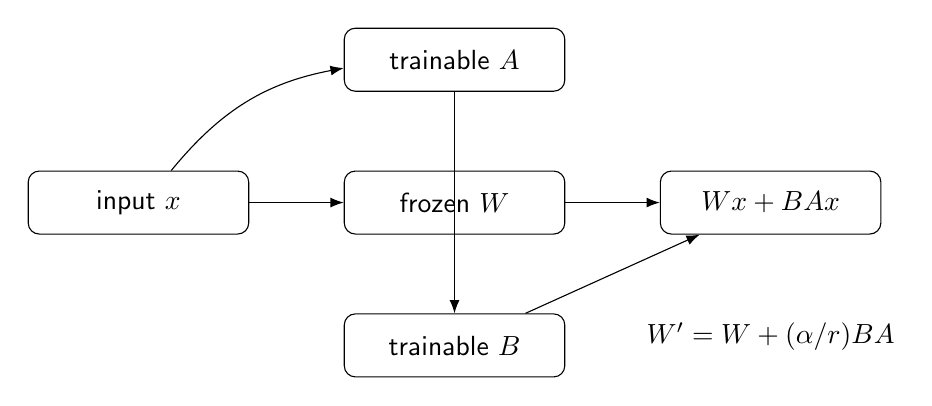
\begin{tikzpicture}[font=\sffamily,>=Latex,box/.style={draw,rounded corners,align=center,minimum width=2.8cm,minimum height=.8cm}]\node[box](x){input $x$};\node[box,right=1.2cm of x](w){frozen $W$};\node[box,above=1cm of w](a){trainable $A$};\node[box,below=1cm of w](b){trainable $B$};\node[box,right=1.2cm of w](sum){$Wx + BAx$};\draw[->](x)--(w);\draw[->](x) to[bend left=20] (a);\draw[->](a)--(b);\draw[->](b)--(sum);\draw[->](w)--(sum);\node[below=1cm of sum]{$W' = W + (\alpha/r)BA$};\end{tikzpicture}\end{document}
